\renewcommand*{\arraystretch}{1.1}

\subsection*{BI / read / 15}
\label{section:bi-read-15}

\noindent\begin{tabularx}{\queryCardWidth}{|>{\queryPropertyCell}p{\queryPropertyCellWidth}|X|}
	\hline
	query & BI / read / 15 \\ \hline
%
	title & Social normals
 \\ \hline
%
	pattern & \hfill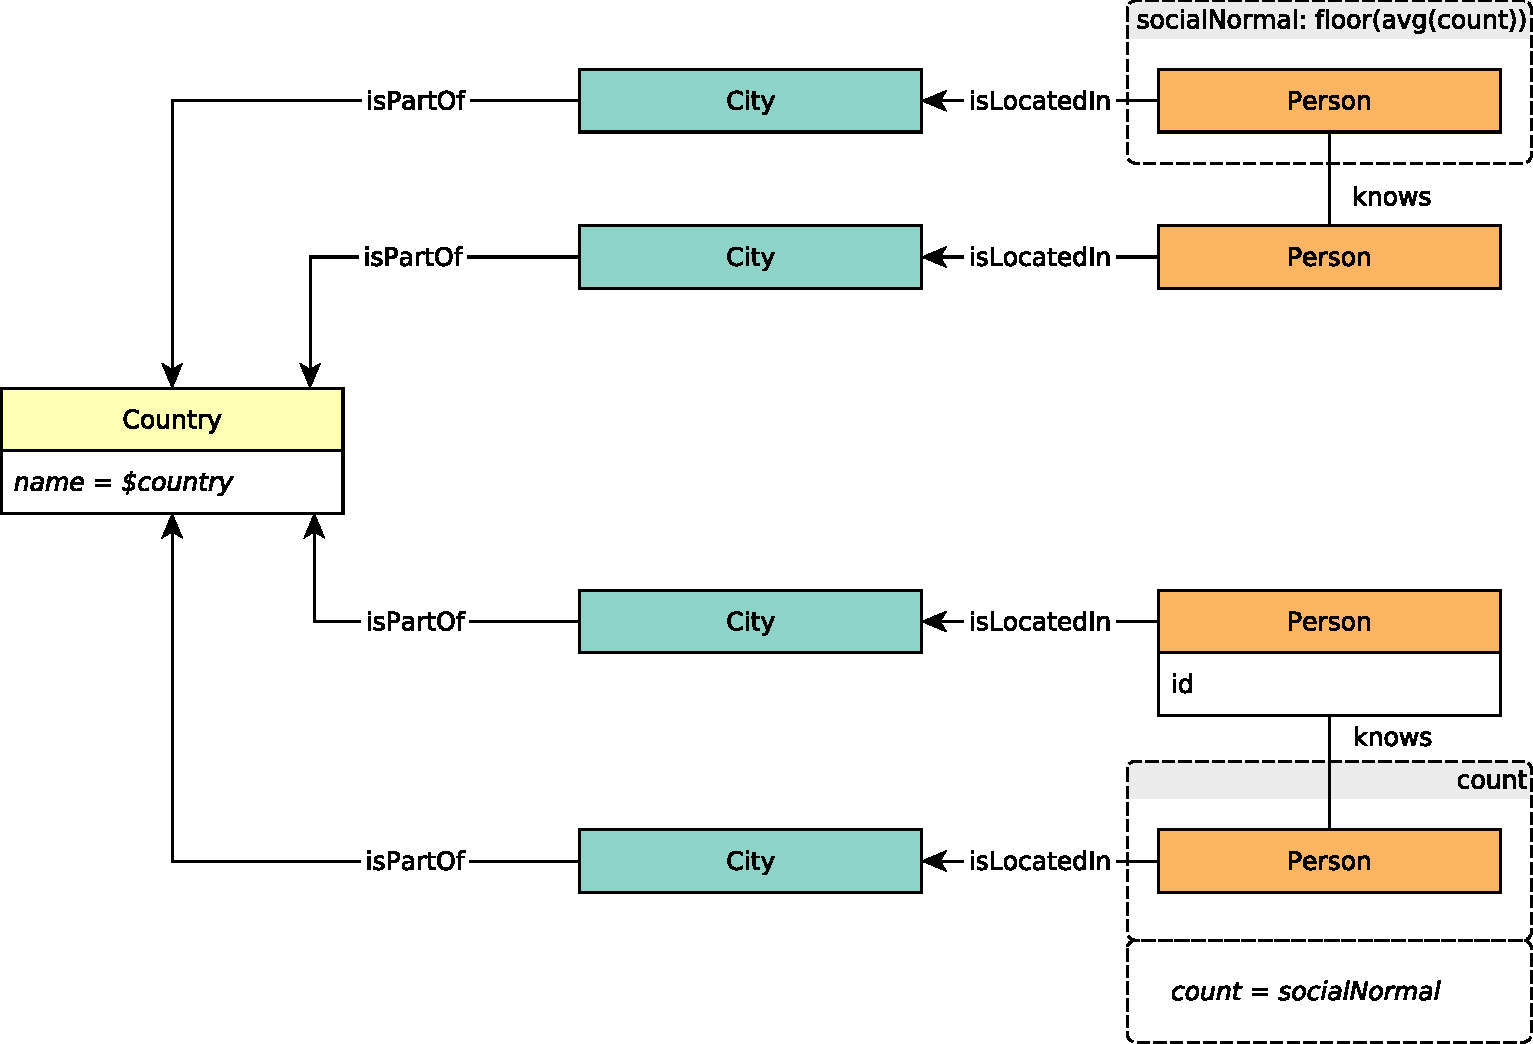
\includegraphics[scale=\patternscale,margin=0cm .2cm]{patterns/bi-read-15}\hfill\vadjust{} \\ \hline
%
	desc. & Given a \texttt{country}, find all \emph{Persons} of the \emph{Country}
whose number of friends in the given \emph{Country} equals the (floor
of) average number of friends that \emph{Persons} of the given
\emph{Country} have in the given \emph{country}.
 \\ \hline
%
	
		params &
		\innerCardVSpace{\begin{tabularx}{\attributeCardWidth}{|>{\paramNumberCell}c|>{\varNameCell}M|>{\typeCell}m{\typeWidth}|Y|} \hline
		$\mathsf{1}$ & country
 & 32-bit Integer
 &  \\ \hline
		\end{tabularx}}\innerCardVSpace \\ \hline
	
%
	
		result &
		\innerCardVSpace{\begin{tabularx}{\attributeCardWidth}{|>{\resultNumberCell}c|>{\varNameCell}M|>{\typeCell}m{\typeWidth}|>{\resultOriginCell}c|Y|} \hline
		$\mathsf{1}$ & person.id
 & 64-bit Integer
 & R &
				 \\ \hline
		$\mathsf{2}$ & count
 & 32-bit Integer
 & R &
				 \\ \hline
		\end{tabularx}}\innerCardVSpace \\ \hline
	
%
	
		sort		&
		\innerCardVSpace{\begin{tabular}{|>{\sortNumberCell}c|>{\varNameCell}l|>{\directionCell}c|} \hline
		$\mathsf{1}$ & person.id
 & $\asc
$ \\ \hline
		\end{tabular}}\innerCardVSpace \\ \hline
	%
	limit & 100 \\ \hline
	%
	CPs &
	\multicolumn{1}{>{\raggedright}l|}{
		\chokePoint{1.2}, 
		\chokePoint{2.3}, 
		\chokePoint{3.2}, 
		\chokePoint{3.3}, 
		\chokePoint{5.3}, 
		\chokePoint{6.1}
		} \\ \hline
	%
	%
\end{tabularx}
\queryCardVSpace